
\documentclass[12pt]{book}

\usepackage [spanish] {babel}
\usepackage [T1]{fontenc}
\usepackage [utf8]{inputenc}
\usepackage {graphicx}
\usepackage{anysize} 
\usepackage[bookmarks=true]{hyperref}
\usepackage{bm} 
%\usepackage{natbib}
\usepackage{color}

\marginsize{4cm}{3cm}{3cm}{4cm}
\usepackage{times}

%No indent document
\setlength\parindent{0pt}

%MY COMMANDS
\definecolor{gray}{rgb}{0.5,0.5,0.2}
\newcommand{\colored}[1]{\textcolor{gray}{\bf #1}}

\newcommand{\bds}[1]{\boldsymbol{ #1 }}
\newcommand{\sub}[1]{\mbox{\scriptsize{#1}}}
\newcommand{\der}[2]{ \frac{ \partial #1 }{\partial #2} }
\newcommand{\dtot}[2]{ \frac{ d #1 }{d #2} }
\newcommand{\pr}[1]{ \left( #1 \right) }
\newcommand{\cor}[1]{ \left[ #1 \right] }
\newcommand{\lla}[1]{ \left\{ #1 \right\} }
\newcommand{\eq}[2]{\begin{equation} \label{#1} #2 \end{equation}}

%CODE COMMANDS============================================================
\newcommand{\python}{\textit{Python} }
\newcommand{\ipython}{\textit{iPython} }
\newcommand{\numpy}{\textit{NumPy} }
\newcommand{\scipy}{\textit{SciPy} }
\newcommand{\matplotlib}{\textit{Matplotlib} }
\newcommand{\mayavi}{\textit{MayaVi2} }
\newcommand{\tkinter}{\textit{TKinter} }

\usepackage{color}
\definecolor{gray97}{gray}{.97}
\definecolor{gray75}{gray}{.75}
\definecolor{gray45}{gray}{.45}

\usepackage{listings}
\lstset{ frame=Ltb,
framerule=0pt,
aboveskip=0.5cm,
framextopmargin=3pt,
framexbottommargin=3pt,
framexleftmargin=0.4cm,
framesep=0pt,
rulesep=.4pt,
backgroundcolor=\color{gray97},
rulesepcolor=\color{black},
%
stringstyle=\ttfamily,
showstringspaces = false,
basicstyle=\small\ttfamily,
commentstyle=\color{gray45},
keywordstyle=\bfseries,
%
numbers=left,
numbersep=15pt,
numberstyle=\tiny,
numberfirstline = false,
breaklines=true,
}

% minimizar fragmentado de listados
\lstnewenvironment{listing}[1][]
{\lstset{#1}\pagebreak[0]}{\pagebreak[0]}

\lstdefinestyle{consola}
{basicstyle=\scriptsize\bf\ttfamily,
backgroundcolor=\color{gray75},
}

\lstdefinestyle{python}
{language=python,
}
%=========================================================================

%#########################################################################
%	FRONT PAGE
%#########################################################################
\begin{document}
\title{Suplemento Computacional \\
\begin{Huge}
\textbf{Electricidad y Magnetismo}
\end{Huge}}
\author{ Sebastian Bustamante Jaramillo\\ \begin{small}
macsebas33@gmail.com
\end{small} \\ \vspace{5cm} \\
\includegraphics[width=3cm]{pictures/UdeA_Shield} \\
Facultad de Ciencias Exactas y Naturales \\ 
Universidad de Antioquia }
\date{}
\maketitle
%#########################################################################



%#########################################################################
%	TABLE OF CONTENTS
%#########################################################################
\newpage{\pagestyle{empty}\cleardoublepage}  

\tableofcontents
\newpage{\pagestyle{empty}\cleardoublepage}  
%#########################################################################



%#########################################################################
%	INTRODUCTION
%#########################################################################

\include{chapters/introduction}

%#########################################################################



%#########################################################################
%	1. ELECTROSTATIC
%#########################################################################

\include{chapters/electrostatic}

%#########################################################################




%#########################################################################
%	2. MAGNETOESTATIC
%#########################################################################

%#########################################################################
\chapter{Magnetostática}
\label{cha:magnetostatic}

%#########################################################################


%*************************************************************************
\section{Ejercicios}
\label{sec:ejercicios}

\
\subsection*{Ejercicio 1 \large{$\pr{\star}$}}

\textbf{Trayectoria en campo no homogéneo}

Considere una partícula de masa $m$ y carga $q$ embebida en un campo 
magnético con la siguiente forma funcional.

\[ \bds B(x, y) = A(x^2+y^2)\bds k \]

Haga un código que utilice la rutina de integración \texttt{RungeKutta4.py} 
de la demostración \ref{sec:DEMO2_03} para integrar la trayectoria de esta 
partícula en el campo $\bds B$. Puede guiarse de la demostración 
\ref{sec:DEMO2_03}, además puede usar valores numéricos de las condiciones 
iniciales, constante $A$, masa $m$ y carga $q$ de su elección.
Finalmente grafique la trayectoria calculada de la partícula cargada y 
realice una animación 3D de la partícula usando la libreria \mayavi.

\textit{Hint:} En la ventana de animación, es conveniente crear una mesa 
con el fin de tener un punto de referencia para notar el movimiento de la 
partícula.

\

\subsection*{Ejercicio 2 \large{$\pr{\star}$}}

\textbf{Billar electrostático con campo magnético}


Considere la demostración \ref{sec:DEMO2_03}. Modifique ambos scripts para
incluir la acción de un campo magnético uniforme y homogéneo que entra hacia
el tablero. La magnitud del campo magnético es de libre elección.


\subsection*{Ejercicio 3 \large{$\pr{\star}$}}

\textbf{Campo magnético de 4 corrientes}

Considere cuatro alambres por los cuales circula una corriente $I_0$, tal
como se muestra en la siguiente figura. Usando la función \texttt{quiver}
de \matplotlib, graficar las líneas de campo magnético en un plano 
perpendicular a las corrientes. Escoja los valores que desee para las 
cantidades del problema.

%.........................................................................
%Charged bar
\begin{figure}[htbp]
	\centering
	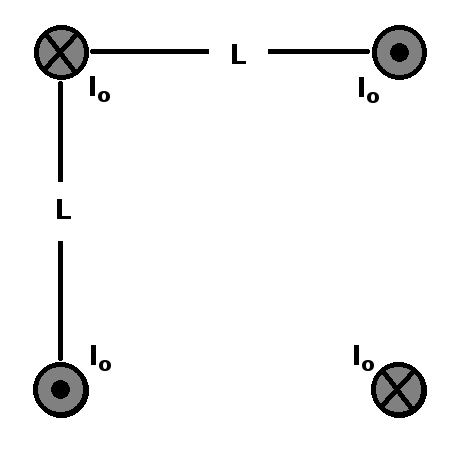
\includegraphics[width=0.4
	\textwidth]
	{./pictures/fourcorrients.png}

	\caption{\small{Cuatro corrientes de igual magnitud.}}
	
	\label{fig:fourcorrients}
\end{figure}
%.........................................................................


\subsection*{Ejercicio 4 \large{$\pr{\star \star}$}}

\textbf{Partícula en un campo dipolar}

Considere una particula cargada en un campo magnetico dipolar, integre 
numéricamente usando la rutina de integración \texttt{RungeKutta4.py} la 
trayectoria de la partícula. Realice los siguiente numerales

\
\begin{itemize}
\item [\textbf{a)}] Grafique usando la función \texttt{quiver} de \matplotlib las 
líneas de campo magnético.
\item [\textbf{b)}] Encuentre una condición inicial (velocidad y posición) para
la cual la partícula interactúe apreciablemente con el campo magnético.
Una interacción interesante puede ser el confinamiento de la trayectoria en
zonas cercanas a los polos del dipolo (Este fenómeno explica las auroras 
boreales). Guarde la trayectoria obtenida en un archivo de texto con el formato
\texttt{[x, y, z, vx, vy, vz]}.  
\item[\textbf{c)}] Realice una animación 3D usando \mayavi donde ilustre el 
movimiento de la partícula cargada.

\textit{Hint:} En la ventana de animación, es conveniente crear un objeto
con el fin de tener un punto de referencia para notar el movimiento de la 
partícula. Este objeto puede ser una esfera en el centro del campo dipolar.

\end{itemize}

Escoja los valores que desee para las cantidades físicas del problema.

%*************************************************************************

%#########################################################################




%#########################################################################
%	3. INDUCTANCE
%#########################################################################

%#########################################################################
\chapter{Electrodinámica}
\label{cha:inductance}

La electrodinámica aborda la evolución temporal de sistemas donde 
interactúan campos magnéticos y eléctricos y cargas en movimiento. En este
caso se tratan temas como la ley de inducción de Faraday y posibles 
aplicaciones, circuitos RL, LC, corriente alterna, etc.

%#########################################################################


\
%*************************************************************************
\section{Demostración 1: Bobina fonocaptora}
\label{sec:DEMO2_01}
\rule{14cm}{0.5mm}

%.........................................................................
%Fonocaptor
\begin{figure}[htbp]
	\centering
	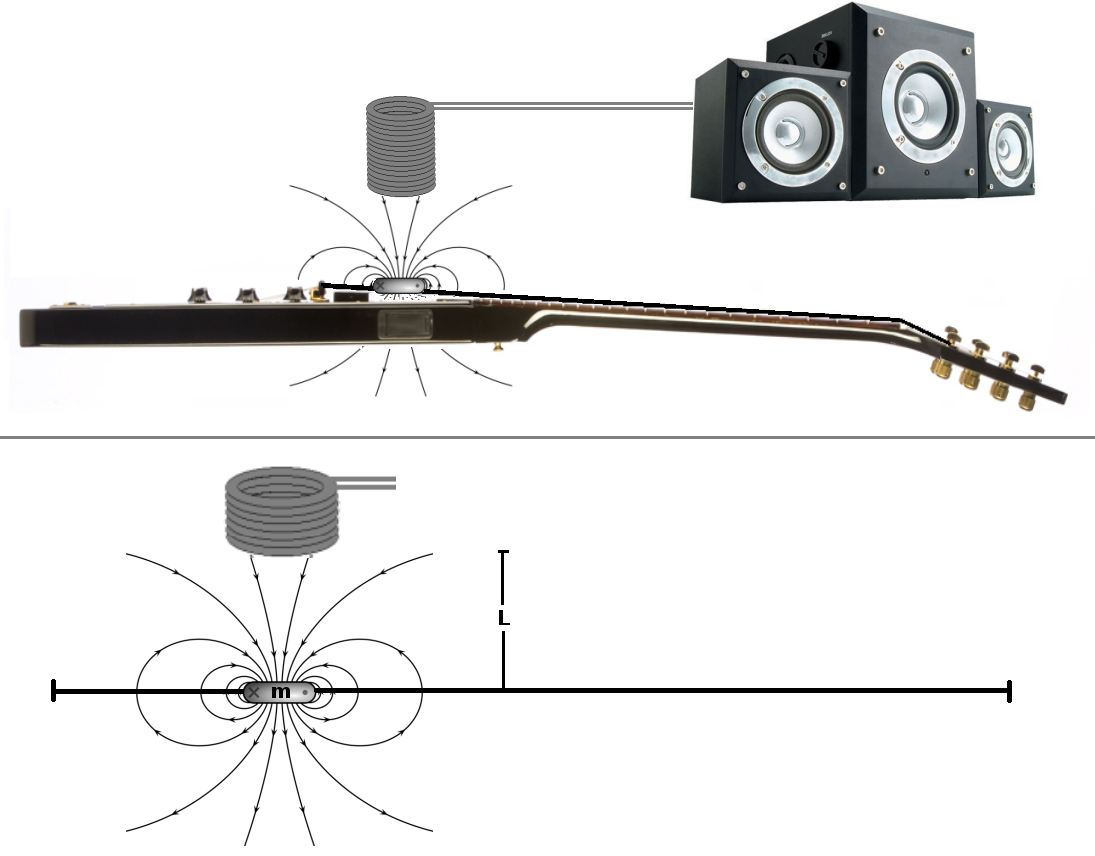
\includegraphics[width=0.65\textwidth]
	{./pictures/fonocaptor.png}

	\caption{\small{Bobina fonocaptora.}}
	
	\label{fig:fonocaptor}
\end{figure}
%.........................................................................

Una interesante aplicación del fenómeno de inducción es la bobina 
fonocaptora. Este dispositivo permite la amplificación del sonido en una 
guitarra eléctrica a partir de la corriente de inducción generada en una 
bobina. Un montaje ilustrativo del experimento puede verse en la figura 
\ref{fig:fonocaptor}.

\

El funcionamiento de este dispositivo se explica a continuación. La cuerda
de la guitarra tiene un material que puede ser magnetizado por un campo 
externo permanente, creando así un momento dipolar inducido y por tanto
un campo magnético dipolar de la forma

%.........................................................................
%Dipole magnetic field
\eq{eq:dipole} 
{\bds B(\bds r) = \frac{\mu_0}{4 \pi}\pr{ \frac{ 3\bds r (\bds m \cdot
\bds r)}{r^5} - \frac{\bds m}{r^3} }}
%.........................................................................

\

Por simplicidad, y teniendo en cuenta que la mayor contribución al flujo 
magnético a través de la bobina es debida a la componente vertical del 
campo magnético, se puede reescribir el campo dipolar como

%.........................................................................
%Aproximated dipole magnetic field
\eq{eq:dipole_approx} 
{\bds B(\bds r) \approx \frac{\mu_0}{2 \pi}{\frac{m}{r^3} }\bds u_j}
%.........................................................................
donde el vector unitario $\bds u_j$ se ha definido perpendicular a la 
cuerda en reposo y apuntando hacia la bobina.

\

Para la cuerda, se asumirá que tiene extremos fijos, de tal forma que la 
solución de onda tiene la forma 

%.........................................................................
%String solution
\eq{eq:string} 
{y(x,t) = y_0(t)\sin\cor{ 2\pi \pr{ f_1t - \frac{x}{\lambda_1} } }}
%.........................................................................
donde $y_0(t) = y_i e^{-t/\tau}$, con $y_i$ la amplitud inicial y $\tau$
el tiempo de vida media de la oscilación, $f_1$ y $\lambda_1$ la frecuencia
y longitud de onda fundamental, $t$ el tiempo y $x$ la coordenada horizontal
definida sobre la cuerda.

\

La frecuencia y longitud de onda fundamental en una cuerda con extremos 
fijos está dada por

%.........................................................................
%Fundamental
\eq{eq:fundamental} 
{f_1 = \frac{ 1}{2D}v \ \ \ \ \ \ \ \lambda_1 = \frac{2D}{n}\ \ \ \ \ \ \ 
v = \sqrt{ \frac{T}{\mu} }}
%.........................................................................
donde $v$ es la velocidad de la onda en la cuerda, $D$ la longitud, $T$ la
tensión y $\mu$ la densidad lineal.

\

Puesto que solo interesa evaluar la oscilación de la cuerda donde está 
ubicado el material magnetizado, se puede reducir la expresión \ref{eq:string}
a

%.........................................................................
%string evaluated on the magnetized material location
\eq{eq:definitive_string} 
{y_m(t) = y(x_m,t) = y_0(t)\sin\cor{ 2\pi f_1t + \delta} }
%.........................................................................
donde $y_m$ es la amplitud de la onda evaluada en la posición del material
magnetizado $x_m$, y sin pérdida de generalidad, la fase obtenida $\delta$
se puede hacer nula $\delta = 0$.

\

El campo magnético medido en la ubicación de la espira debido al material
magnetizado sobre la cuerda es 

%.........................................................................
%Aproximated dipole magnetic field with the vibrating string
\eq{eq:final_b} 
{\bds B(\bds r) \approx \frac{\mu_0}{2 \pi}{\frac{m}{[L-y_m(t)]^3} }\bds u_j}
%.........................................................................

Calculando el potencial inducido en la bobina fonocaptora, se obtiene
%.........................................................................
%Induced potential
\begin{eqnarray}
V_{fem} &=& N\dtot{\phi}{t} = NA\dtot{B}{t} \\
&=& NA \frac{3\mu_0}{2 \pi}{\frac{m}{[L-y_m(t)]^4} }\dtot{y_m(t)}{t}
\end{eqnarray}
%.........................................................................


Usando la expresión para la amplitud de la oscilación en la cuerda se llega
a

%.........................................................................
%Induced potential
\begin{eqnarray}
\frac{V_{fem}}{V_0 } = 
\cor{ 1 - \frac{y_0}{L}\sin( 2\pi f_1 t ) }^{-4}\frac{y_0}{L}
e^{-t/\tau}\cor{ 2\pi f_1 \cos(2\pi f_1 t) - \frac{1}{\tau}\sin( 2\pi f_1 t ) }
\end{eqnarray}
%.........................................................................
donde se ha definido el potencial de referencia $V_0$ como

\[ V_0 = \frac{3\mu_0 NAm }{2\pi L^3} \]

A continuación se ilustra el código para el cálculo del problema 
%ccccccccccccccccccccccccccccccccccccccccccccccccccccccccccccccccccccccccc
%DEMO 2_01
\begin{listing}[style=python]
#!/usr/bin/env python
#==========================================================
# DEMOSTRACION 1:
# Bobina fonocaptora
#==========================================================
import numpy as np
import matplotlib.pylab as plt
import AudioLib as ad

#Funcion de oscilacion original
def y(t):
    return y0*np.exp(-t/tau)*np.sin( 2*np.pi*freq1*t )

#Funcion de potencial inducido por bobina fonocaptora
def Vfem(t):
    return (1-y0/L*np.sin( 2*np.pi*freq1*t ))**-4*y0/L*\
    np.exp( -t/tau )*( 2*np.pi*freq1*\
    np.cos( 2*np.pi*freq1*t ) - \
    1/tau*np.sin( 2*np.pi*freq1*t ) )


#CONSTANTES
#Frecuencia fundamental de la cuerda [Hz]
freq1 = 440.
#Amplitud maxima de oscilacion de la cuerda [m]
y0 = 0.002
#Longitud de la cuerda [m]
L = 0.7
#Tiempo de vida medio de una oscilacion [s]
tau = 1.

#Tiempo maximo [s]
tmax = 5
#Intervalos
dt = 1/44100.
#Arreglo de tiempo 
tiempo = np.arange( 0, tmax, dt )

#Potencial
V = Vfem( tiempo )
#Oscilacion original
y_cuerda = y( tiempo )

#Grafica
plt.plot( tiempo, V, linewidth = 0.5 )
plt.grid()
plt.title( "Potencial inducido por una bobina fonocaptora")
plt.xlabel( "t [s]" )
plt.ylabel( "Potential [V_0]" )
plt.show()

#Audio producido por la bobina
nota_bobina = ad.audio()
nota_bobina.load( V*ad.Amplitude/max(V) )
nota_bobina.play()

#Audio original de la cuerda
nota_cuerda = ad.audio()
nota_cuerda.load( y_cuerda*ad.Amplitude/max(y_cuerda) )
nota_cuerda.play()
\end{listing}
%ccccccccccccccccccccccccccccccccccccccccccccccccccccccccccccccccccccccccc


El resultado que se obtiene es


%.........................................................................
%Trayectories
\begin{figure}[htbp]
	\centering
	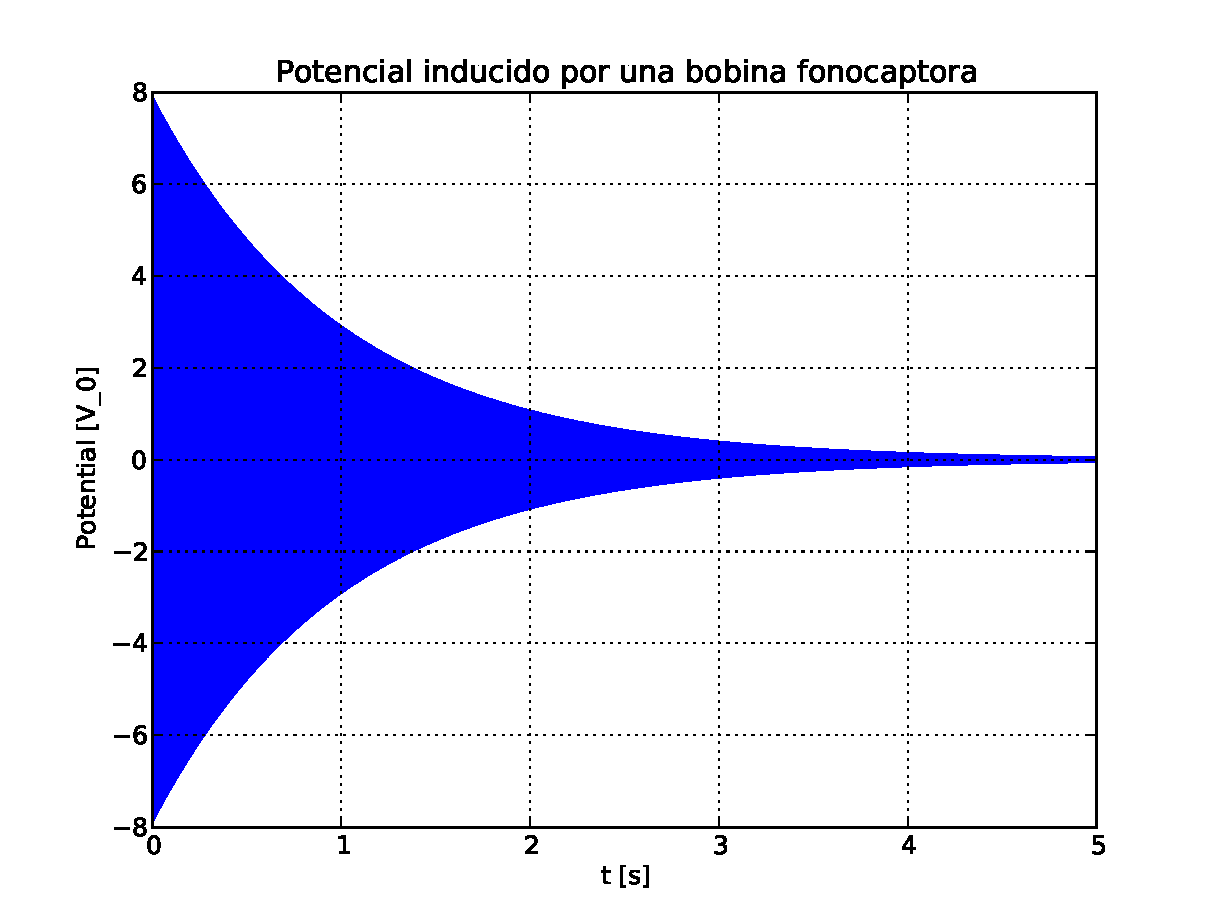
\includegraphics[width=0.8\textwidth]
	{./pictures/demo4_01.pdf}

	\caption{\small{Potencial de inducción producido por una bobina
	fonocaptora.}}
	
	\label{fig:fono_fem}
\end{figure}
%.........................................................................


El potencial obtenido es una función oscilante con la misma frecuencia de
la cuerda original, lo que permite entonces digitalizar el sonido de la 
guitarra. Ambos sonidos son recreados por el código anterior, primero el 
sonido producido por un parlante conectado a la bocina y el segundo, el
sonido producido por la guitarra originalmente.

\

A continuación se explica cada parte del código


%ccccccccccccccccccccccccccccccccccccccccccccccccccccccccccccccccccccccccc
%DEMO 4_01
\begin{listing}[style=python, numbers = none]
import numpy as np
import matplotlib.pylab as plt
import AudioLib as ad
\end{listing}
%ccccccccccccccccccccccccccccccccccccccccccccccccccccccccccccccccccccccccc
Se importan las librerías estándar más la librería \texttt{AudioPy.py} con
el alias de \texttt{ad}. Esta librería se anexa en la sección de códigos de
la parte del curso y permite la manipulación de audio desde \python. En 
orden para correr el código de la demostración apropiadamente, es 
necesario instalar el paquete \texttt{pyaudio}

%.........................................................................
%Installing pyaudio
\begin{listing}[style=consola, numbers=none]
\$ sudo apt-get install python-pyaudio
\end{listing}
%.........................................................................

%ccccccccccccccccccccccccccccccccccccccccccccccccccccccccccccccccccccccccc
%DEMO 4_01
\begin{listing}[style=python, numbers = none]
#Funcion de oscilacion original
def y(t):
    return y0*np.exp(-t/tau)*np.sin( 2*np.pi*freq1*t )

#Funcion de potencial inducido por bobina fonocaptora
def Vfem(t):
    return (1-y0/L*np.sin( 2*np.pi*freq1*t ))**-4*y0/L*\
    np.exp( -t/tau )*( 2*np.pi*freq1*\
    np.cos( 2*np.pi*freq1*t ) - \
    1/tau*np.sin( 2*np.pi*freq1*t ) )
\end{listing}
%ccccccccccccccccccccccccccccccccccccccccccccccccccccccccccccccccccccccccc
Definición de las funciones usadas en el código. La primera, \texttt{y(t)},
es la función de oscilación de la guitarra (expresión 
\ref{eq:definitive_string}) y la segunda, \texttt{Vfem(t)}, es la función 
de potencial inducido para la bobina.

%ccccccccccccccccccccccccccccccccccccccccccccccccccccccccccccccccccccccccc
%DEMO 4_01
\begin{listing}[style=python, numbers = none]
#CONSTANTES
#Frecuencia fundamental de la cuerda [Hz]
freq1 = 440.
#Amplitud maxima de oscilacion de la cuerda [m]
y0 = 0.002
#Longitud de la cuerda [m]
L = 0.7
#Tiempo de vida medio de una oscilacion [s]
tau = 1.

#Tiempo maximo [s]
tmax = 5
#Intervalos
dt = 1/44100.
#Arreglo de tiempo 
tiempo = np.arange( 0, tmax, dt )

#Potencial
V = Vfem( tiempo )
#Oscilacion original
y_cuerda = y( tiempo )
\end{listing}
%ccccccccccccccccccccccccccccccccccccccccccccccccccccccccccccccccccccccccc
En esta parte se definen las variables físicas del problema, incluyendo la
frecuencia de oscilación de la guitarra \texttt{freq1}, la amplitud de la 
cuerda \texttt{y0}, la longitud \texttt{L} y el tiempo de vida medio de la
oscilación \texttt{tau}. Luego se definen los parámetros relacionados con 
el tiempo de muestreo de la señal del potencial, esto es, tiempo máximo
\texttt{tmax} en segundos, paso de tiempo \texttt{dt} \footnote{Este valor
es estándar para la generación de señales de audio y no debe cambiarse.},
y el arreglo de tiempo \texttt{tiempo}, el cual se crea usando la función
\texttt{arange} de la librería \numpy. Finalmente se calcula el array con
la información del potencial inducido en el tiempo como \texttt{V = Vfem
( tiempo )} y la oscilación de la cuerda originalmente \texttt{y\_cuerda = 
y( tiempo )}.


%ccccccccccccccccccccccccccccccccccccccccccccccccccccccccccccccccccccccccc
%DEMO 4_01
\begin{listing}[style=python, numbers = none]
#Grafica
plt.plot( tiempo, V, linewidth = 0.5 )
plt.grid()
plt.title( "Potencial inducido por una bobina fonocaptora")
plt.xlabel( "t [s]" )
plt.ylabel( "Potential [V_0]" )
plt.show()
\end{listing}
%ccccccccccccccccccccccccccccccccccccccccccccccccccccccccccccccccccccccccc
Se grafica el potencial inducido vs el tiempo usando la librería 
\matplotlib.


%ccccccccccccccccccccccccccccccccccccccccccccccccccccccccccccccccccccccccc
%DEMO 4_01
\begin{listing}[style=python, numbers = none]
#Audio producido por la bobina
nota_bobina = ad.audio()
nota_bobina.load( V*ad.Amplitude/max(V) )
nota_bobina.play()

#Audio original de la cuerda
nota_cuerda = ad.audio()
nota_cuerda.load( y_cuerda*ad.Amplitude/max(y_cuerda) )
nota_cuerda.play()
\end{listing}
%ccccccccccccccccccccccccccccccccccccccccccccccccccccccccccccccccccccccccc
Finalmente se crean los audios correspondientes a la guitarra y a la bobina.
Para esto se usa la clase \texttt{audio} de la librería \texttt{AudioLib} 
(\texttt{ad}). Primero se crea el objeto \texttt{nota\_bobina}, luego, usando
el método \texttt{nota\_bobina.load}, se carga la señal para este audio.
Para esto se normaliza la señal con el máximo valor que toma la amplitud del
potencial \texttt{max(V)} \footnote{A pesar de que esta señal es un potencial,
se puede modelar un parlante como una resistencia, de tal forma que la señal
sonora es proporcional al potencial.}, y luego se multiplica por la amplitud
\texttt{ad.Amplitude} que corresponde al máximo volumen que puede reproducir
un computador, este valor es estándar y está almacenado en la librería 
\texttt{AudioLib}. Ahora, usando el método \texttt{nota\_bobina.play()} se
reproduce el audio.

Se realiza el mismo procedimiento para la señal de la guitarra.


\rule{14cm}{0.5mm}
%*************************************************************************


%*************************************************************************
\section{Ejercicios}
\label{sec:ejercicios}

\
\subsection*{Ejercicio 1 \large{$\pr{\star}$}}

\textbf{Bobina fonocaptora con armónicos}

Para simular de forma realista el sonido de una guitarra se deben considerar
los armónicos de orden superior, esto es, cuando se reproduce una cierta
nota en una guitarra, y en general en cualquier instrumento musical, no solo
se reproduce esa nota específica sino un conjunto de notas con frecuencias
que son múltiplos de la frecuencia fundamental, estas notas se denominan 
armónicos. 

\

Considere el mismo ejercicio de la demostración 1 pero incluya los primeros
4 armónicos. Para esto sume a la amplitud de la guitarra 4 notas sinusoidales
con frecuencias multiplos de la frecuencia fundamental, es decir

\[ \omega_n = n \times \omega_1,\ \ \ \ \ \ n=1,2,3,4 \]

con $\omega_1$ la frecuencia escogida (En la demostración 1 se ha tomado 
$440$ Hz). Escoja las amplitudes relativas de cada armónico como desee, pero
manteniendo siempre la frecuencia fundamental con mayor amplitud. 

\

Al igual que la demostración 1, grafique el potencial inducido y reproduzca
los audios de la bobina y de la guitarra.

\

\subsection*{Ejercicio 2 \large{$\pr{\star}$}}

\textbf{Gravímetro magnético}

\

Una interesante aplicación del fenómeno de inducción magnética es el
gravímetro magnético. Su funcionamiento se basa en la caída de un cuerpo
magnetizado con un campo dipolar y al pasar por cada espira se registra un
pico en la corriente del amperímetro debido a inducción magnética, tal
como se muestra en la siguiente figura.

\newpage
%.........................................................................
%Gravimeter
\begin{figure}[htbp]
	\centering
	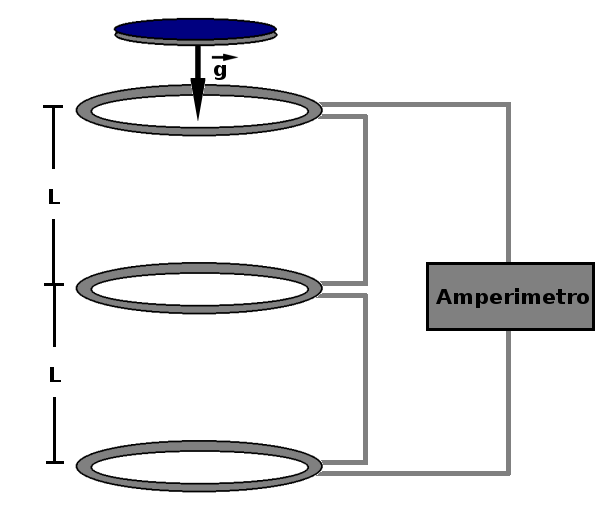
\includegraphics[width=0.6\textwidth]
	{./pictures/gravimeter.png}

	\caption{\small{Gravímetro magnético.}}
	
	\label{fig:gravimeter}
\end{figure}
%.........................................................................

Basado en esto, realice un código que simule la señal de la corriente de 
inducción medida en función del tiempo a medida que el cuerpo cae. 

\textit{Hint:} para el campo magnético del cuerpo, asuma un campo con la 
aproximación de la ecuación \ref{eq:dipole_approx}, donde la dirección
$\bds u_j$ se toma en dirección vertical hacia arriba.


\

\subsection*{Ejercicio 3 \large{$\pr{\star}$}}

\textbf{Inducción por deslizamiento}

\

Considere la situación de la siguiente figura

%.........................................................................
%Induction by fall
\begin{figure}[htbp]
	\centering
	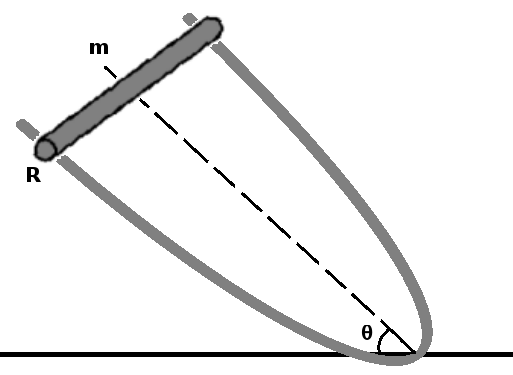
\includegraphics[width=0.5\textwidth]
	{./pictures/induction.png}

	\caption{\small{Inducción por deslizamiento.}}
	
	\label{fig:induction_fall}
\end{figure}
%.........................................................................

Se tiene un cilindro macizo conductor de radio $R$ y masa $m$ que rueda sin
deslizar desde una altura $h$ sobre una base de forma parabólica también 
conductora y que está inclinada un ángulo $\theta$ respecto a la horizontal.

\

Realice un código que grafique el potencial inducido en función del tiempo
mientras el cilindro rueda. \textit{Hint:} asigne los valores numéricos y
físicos que desee, además de los parámetros geométricos de la parábola.



%*************************************************************************

%#########################################################################

\begin{thebibliography}{}
\bibitem[1]{purcell} Purcell E. M. Electricity and Magnetism, Berkeley 
Physics Course Vol. 2. Mc Graw Hill. 1965. 
\bibitem[2]{finn} Alonso \& Finn. Física, Campos y Ondas Vol. 2. Addison-Wesley. 
1998.
\bibitem[3]{sears} Sears, Zemanski, Young \& Freedman, Física Universitaria Vol. 2. 
Pearson Addison-Wesley, 11 ed, 2004.
\end{thebibliography}

\end{document}